\section{实验结果}
\subsection{在UNIX V6++中添加一个新的系统调用方法的主要步骤}
主要步骤如下:
\begin{enumerate}
    \item 在\texttt{SystemCall.h}中添加新的系统调用方法的声明
    \item 在\texttt{SystemCall.cpp}中添加新的系统调用方法的实现,并在SystemCallTableEntry中选择一项,将其修改为\verb|{参数量,&新方法名称}|
\end{enumerate}
要注意的是,即使参数量不为零,在声明和实现中的参数表都为空。因此推荐在注释中记录相关信息。

\subsection{系统调用过程中核心栈的变化}
表\ref{table2}为系统调用准备好返回值时的核心栈情况。图\ref{3vs2},\ref{2vs1}为沿时间轴反方向的核心栈相对变化情况。

从图\ref{3vs2}中可以看出,主要有三点变化:
\begin{enumerate}
    \item \texttt{u\_ar0}指向的核心栈中保存\texttt{EAX}单元由\texttt{0xFFFFFFFF}变为\texttt{0x00000001};
    \item 局部变量\texttt{i}初始化,并累加至\texttt{0x00000064};
    \item 地址\texttt{0xC03FFF44}内的值变为\texttt{Sys\_Getppid}的栈帧\texttt{EBP},推测是由于调用\texttt{Kernel::Instance().GetProcessManager()},\texttt{Kernel::Instance().GetUser()}所遗留下来的栈帧。
\end{enumerate}

图\ref{2vs1}中体现出的变化为\texttt{u\_ar0}指向的核心栈中保存\texttt{EAX}单元由\texttt{Sys\_Getppid}对应的系统调用号\texttt{0x00000031}变为\texttt{0xFFFFFFFF},即-1。

\begin{table*}[htbp]
\vspace{-3.6mm}
    \centering
    \begin{threeparttable}[b]
     \begin{tabular}{cllc}\toprule
           地址    &\texttt{\texttt{核心栈内容}}&说明&\\\midrule
\texttt{0xC03FFF2C}&\texttt{0x00000002}&局部变量\texttt{curpid}    &  \multirow{7}{*}{\texttt{Sys\_Getppid}栈帧}\\
\texttt{0xC03FFF30}&\texttt{0xC03FF000}&   局部变量,指向\texttt{User}结构的指针     & \\
\texttt{0xC03FFF34}&\texttt{0xC0120AA0}&        & \\
\texttt{0xC03FFF38}&\texttt{0x00000064}&局部变量\texttt{i}& \\
\texttt{0xC03FFF3C}&\texttt{0xC011C9E0}&        & \\
\texttt{0xC03FFF40}&\texttt{0x00000400}&        & \\
\texttt{0xC03FFF44}&\texttt{0xC03FFF64}&\texttt{Trap1}栈帧EBP        & \\
\texttt{0xC03FFF48}&\texttt{0xC01075CC}&\texttt{Trap1}调用\texttt{Sys\_Getppid}的返回地址        & \\\midrule
\texttt{0xC03FFF4C}&\texttt{0x00000020}&        & \multirow{9}{*}{\texttt{Trap1}栈帧}\\
\texttt{0xC03FFF50}&\texttt{0x00000020}&        & \\
\texttt{0xC03FFF54}&\texttt{0xC03FFF94}&        & \\
\texttt{0xC03FFF58}&\texttt{0xC03FF000}&  局部变量,指向\texttt{User}结构的指针     & \\
\texttt{0xC03FFF5C}&\texttt{0x00000020}&        & \\
\texttt{0xC03FFF60}&\texttt{0x00000002}&        & \\
\texttt{0xC03FFF64}&\texttt{0xC03FFF94}& \texttt{Trap}栈帧EBP       & \\
\texttt{0xC03FFF68}&\texttt{0xC01074E1}& \texttt{Trap}调用\texttt{Trap1}的返回地址       & \\
\texttt{0xC03FFF6C}&\texttt{0xC0107FF8}& \texttt{Trap}所需参数\texttt{callp->call},即\texttt{Sys\_Getppid}地址  & \\\midrule
\texttt{0xC03FFF70}&\texttt{0xC0202000}&        & \multirow{13}{*}{\makecell[l]{系统调用处理程序\\\texttt{Trap}栈帧}}\\
\texttt{0xC03FFF74}&\texttt{0xC03FFF94}&        & \\
\texttt{0xC03FFF78}&\texttt{0xC01073DF}&        & \\
\texttt{0xC03FFF7C}&\texttt{0xC0117F48}&  指向系统调用表中\texttt{Sys\_Getppid}所在项地址的指针      & \\
\texttt{0xC03FFF80}&\texttt{0xC03FF000}&  局部变量,指向\texttt{User}结构的指针      & \\
\texttt{0xC03FFF84}&\texttt{0x00000001}&  局部变量\texttt{i}  & \\
\texttt{0xC03FFF88}&\texttt{0xC03FFFB8}&  指向系统调用传入参数的起始地址的指针      & \\
\texttt{0xC03FFF8C}&\texttt{0xC011C9E0}&        & \\
\texttt{0xC03FFF90}&\texttt{0x00109A97}&        & \\
           \texttt{0xC03FFF94}&\texttt{0xC03FFFE8}& 系统调用入口程序栈帧EBP&\\
           \texttt{0xC03FFF98}&\texttt{0xC0107360}& 系统调用入口程序调用\texttt{Trap}的返回地址    \\
           \texttt{0xC03FFF9C}&\texttt{0xC03FFFA4}&指向软件现场起始地址的指针\\
           \texttt{0xC03FFFA0}&\texttt{0xC03FFFEC}&指向硬件现场起始地址的指针 \\\midrule
           \texttt{0xC03FFFA4}&\texttt{0x00000000}&GS  &\multirow{11}{*}{软件现场} \\
           \texttt{0xC03FFFA8}&\texttt{0x00000000}&FS   \\
           \texttt{0xC03FFFAC}&\texttt{0x00000023}&DS   \\
           \texttt{0xC03FFFB0}&\texttt{0x00000023}&ES   \\
           \texttt{0xC03FFFB4}&\texttt{0x00000002}&EBX,传入系统调用函数的第一个参数\texttt{pid}\tnote{$\dagger$}  \\
           \texttt{0xC03FFFB8}&\texttt{0x00000001}&ECX  \\
           \texttt{0xC03FFFBC}&\texttt{0x00000002}&EDX  \\
           \texttt{0xC03FFFC0}&\texttt{0x00000000}&ESI  \\
           \texttt{0xC03FFFC4}&\texttt{0x00007E00}&EDI  \\
           \texttt{0xC03FFFC8}&\texttt{0xC03FFFE8}&系统调用入口程序栈帧EBP  \\
           \texttt{0xC03FFFCC}&\texttt{0x00000001}&EAX,系统调用函数返回值  \\\midrule
           \texttt{0xC03FFFD0}&\texttt{0x00000001}&  \multirow{6}{*}{系统调用入口程序局部变量区}    &\multirow{7}{*}{程序调用入口程序栈帧}\\
           \texttt{0xC03FFFD4}&\texttt{0xC03FF000}&    \\
           \texttt{0xC03FFFD8}&\texttt{0xC0124984}&     \\
           \texttt{0xC03FFFDC}&\texttt{0xC03FFFEC}&     \\
           \texttt{0xC03FFFE0}&\texttt{0xC0007E00}&     \\
           \texttt{0xC03FFFE4}&\texttt{0xC0007E00}&     \\
           \texttt{0xC03FFFE8}&\texttt{0x007FFFA8}&用户态程序getppid栈帧的EBP,见图\ref{int80}\\\midrule
           \texttt{0xC03FFFEC}&\texttt{0x00403580}&EIP,\texttt{int 80}后一条汇编语句的地址,见图\ref{disammble}  &\multirow{5}{*}{硬件现场}\\
            \texttt{0xC03FFFF0}&\texttt{0x0000001}&CS   \\
            \texttt{0xC03FFFF4}&\texttt{0x00000202}&EFLAGS\\
            \texttt{0xC03FFFF8}&\texttt{0x007FFF94}&ESP,见图\ref{int80}  \\
            \texttt{0xC03FFFFC}&\texttt{0x00000023}&SS   \\
            \multicolumn{4}{c}{核心栈栈底}\\
        \bottomrule
    \end{tabular}
    \begin{tablenotes}
    \footnotesize
    \item[$\dagger$]{图\ref{test}中在运行\texttt{getppid}之前先运行了\texttt{ls}函数,使得传入的\texttt{pid}为3,而在后续的调试过程中,没有运行\texttt{ls},使得传入的\texttt{pid}为2}
    \end{tablenotes}
    \end{threeparttable}
    \caption{系统调用准备好返回值时u\_ar0所指内存地址附近的内存单元}\label{table2}
    \end{table*}
    \begin{figure}[!htbp]
        \centering
        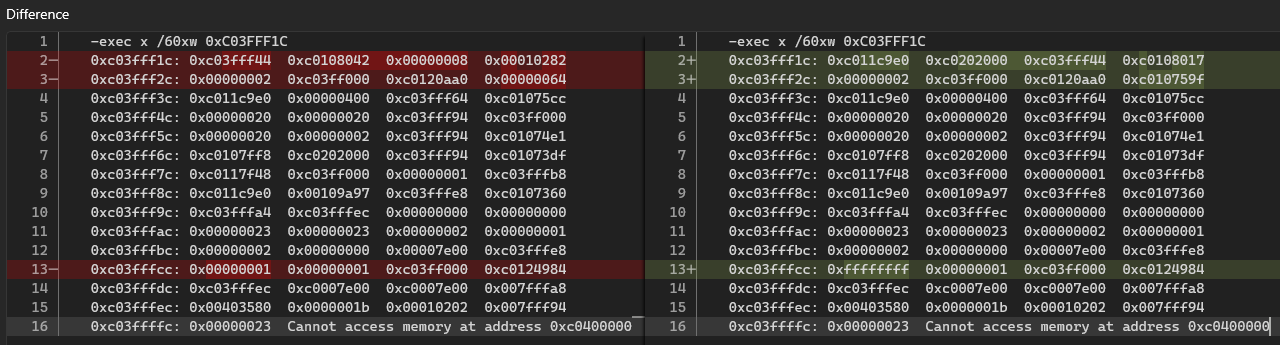
\includegraphics[width=\textwidth]{images/3vs2.png}
        \caption{系统调用准备好返回值时(左)与线性查找开始时(右)的核心栈的对比}\label{3vs2}
    \end{figure}
    
 \begin{figure}[!htbp]
        \centering
        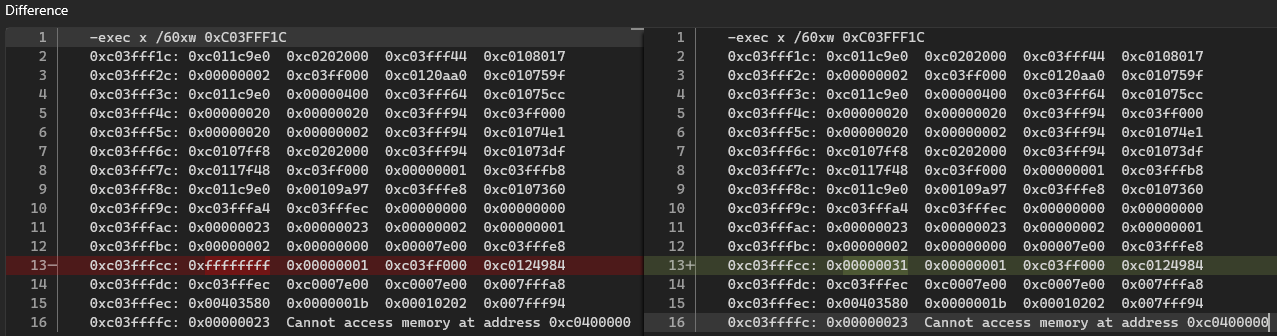
\includegraphics[width=\textwidth]{images/2vs1.png}
        \caption{线性查找开始时(左)与进入系统调用时(右)的核心栈的对比}\label{2vs1}
    \end{figure}
    